\section{Pulse Oximeter (Hearbeat Monitor)}
In researching ways to detect the human heartbeat, we found that photoplethysmography would be the simplest and least expensive way to bring an immediate and personal touch to the gallery installation. A photoplethysmograph is usually obtained with a pulse oximeter - this is the same device that grips a person's finger in hospitals to measure the heart \& respiration rates. 

\paragraph{Concepts}
A pulse oximeter simply illuminates the skin with light from an LED (usually infrared), and measures the luminances of the skin on the other side. Each cardiac cycle brings more blood to the extremeties, and thus the finger is denser and less light passes through to the detector. When the blood flows away, more light is let through. This fluctuation can be recorded and the timing of the luminance peaks used for recording the heart rate.

This project required knowledge of photoplethysmography \cite{PO} \cite{EC1}, signal processing filters \cite{EC2} and operational amplifiers \cite{HL} \cite{BK} \cite{BB}.

\begin{figure}[htp]\centering
  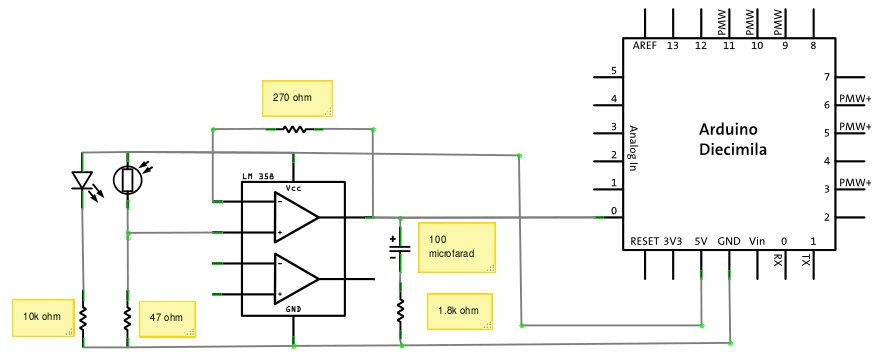
\includegraphics[width=.99\textwidth]{images/schematic-final.png}
  \caption{This is the pulse oximeter schematic!}\label{fig:poschem}
\end{figure}
\paragraph{Implementation}
This device is adventageous for its low intrusiveness. In our implementation, the visitor just needs to gently place their finger on top of the light sensor. Depending on the person, the shape, rate and range of the photoplethysmograph obtained can vary widely, but we found the results distinct enough to obtain a heart rate from almost every participant. 

Our device used the amplified signal of an inexpensive photoresistor passed through a high pass filter and captured by an Arduino microcontroller \cite{ARD}. The microcontroller fed an averaged luminosity to a Processing \cite{P5} sketch on the host computer, which analyzed the signal for peaks. The peaks were then converted to a frequency, and passed along to the gallery software. The software is general to heart rate monitoring, and can be used for other applications that are interested in the data.

\paragraph{}
The electronics schematics are included as both a PDF diagram and as a file for Frizing\cite{FTZ} and can be found in this pacakge at \texttt{/august/doc/heartbeatmonitor}.

The source code for the microcontroller and for computer-side analysis can be found in this package at \texttt{/august/src/gallery/PulseOximeter} and \texttt{/august/src/gallery/WiremapClient} \cite{PACK}.
